\documentclass[11pt]{beamer}
\usepackage[utf8]{inputenc}
\usepackage[T1]{fontenc}
\usepackage{lmodern}
\usetheme[progressbar=frametitle]{metropolis}
\usepackage{graphicx}
\begin{document}
	\title{\textbf{Website Design Ranker}}
	\subtitle{Using Machine Learning}
	%\logo{}
	\institute{\large Department of Computer Science and Engineering \\\textbf{FISAT}}
	\date{16 SEPTEMBER 2019}
	\author{{\scriptsize Adhyaksh Guhan - 7 , Anet Eliza Johny - 23 , Dharwish Raj - 47 , \\ Joel J Padayattil - 60}}
	%\setbeamercovered{transparent}
	%\setbeamertemplate{navigation symbols}{}
	\begin{frame}[plain]
		\maketitle
	\end{frame}
	\begin{frame}{Introduction}
		\begin{itemize}
			
			
			\item Our project is aimed at ranking websites in terms of its design which is evaluated based on certain parameters.
			
			\item Since a perfect model for website ranking  is not in practice this  follows ranking according to submissions by critics.
			
			\item Thus we compare ranking implementation done by Google that analyses a webpage's content.
		
			\item We will be comparing against:
				\item A Website that ranks other design according to submissions by critics
				\item A ranking implementation done by Google that analyses a web-page's contents
		\end{itemize}
	\end{frame}
	\begin{frame}{Problem Statement}
		\begin{itemize}

			\item Our main problem is to evaluate website designs using an algorithm.
			
			\item It must take into account various parts of the website to use as parameters.
			
			\item For example: pepole won't be interested to visit a site if they are berated with ads.Thus ads above a degree will be considered as the parameter for ranking.

			\item There are no existing algorithms or methods that manage to analyze and evaluate websites in this way.
		\end{itemize}
	\end{frame}
	\begin{frame}{Why "Website Design Ranker" ?}
			\begin{itemize}
			\item Website Design Ranker will rank set of input websites based on certain parameters.
			\item It will be helpful to find best website among list of websites which have same content.
			\item We can compare our website design with other competing websites.
			\item We can see how a website's design may improve in an area.

			\end{itemize}
	\end{frame}
	\begin{frame}
	\frametitle{{Related Works : Google Page Layout}}
	\begin{itemize}
		\item Google introduced Page Layout Algorithm to analyze website readability.[1]
		\item Looks for the layout of the web page and the amount of content we see in the page once we click on a result.[1]
		
		\item Focuses to reduce the difficulty of users to find the actual content.[1]
		
		\item  The websites which does not have a lot of visible content above-the-fold and dedicates a large fraction (above a normal degree) to ads will be affected.[1]
		
		
	\end{itemize}

	\end{frame}
	\begin{frame}
\frametitle{{Related Works : Google Page Layout}}
\begin{figure}
	
	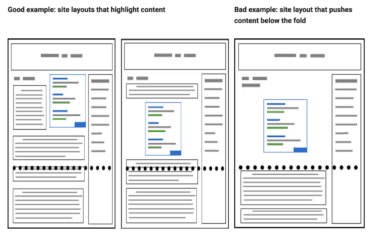
\includegraphics[width=10cm]{image/gpa.png}
	\caption{One of the criteria of GPL Algorithm\textsuperscript{[Fig:1]}}
	\label{fig1:gpa}
\end{figure}
\end{frame}
	\begin{frame}{Proposed System}
\begin{itemize}
	\item Website Design Ranker will rank set of input websites based on certain parameters.
	\item The parameter we are focussing on is color.
	\item Then we move on for public review.
	\item This will be helpful to finding the best website among list of websites.
	\item We can compare our website design with other competing websites.
	\item We can see how a website's design may improve in an area.
	
\end{itemize}
\end{frame}
\begin{frame}
\frametitle{Explanation}
\begin{itemize}
	\item It is an objective analysis of website designs by ranking them based on a parameter.
	\item The website's CSS file is scrapped via a web scrapper and then read through.
	\item The file is then parsed to find hex codes based on a regular expression.
	\item Once the codes are found, they are counted and printed using a variable.
\end{itemize}
\end{frame}
\begin{frame}
\frametitle{Input Data}
\end{frame}
	\begin{frame}
	\frametitle{{Algorithm}}
	\begin{enumerate}
		\item[1.] Start
		\item[2.] Using a website scraper to accept the various website addresses
		\item[3.] Scraping through the source code of each website via CSS files
		\item[4.] Find the hex codes of all elements of the website and count them with a count variable
		\item[5.] If count == 0 then give mark as 0
		\item[6.] else if count > 5 then also give mark as 0
		\item[7.] else if count <= 5 then give mark as 1
		\item[8.] Stop
	\end{enumerate}
	
	\end{frame}
\begin{frame}
\frametitle{Output}
\end{frame}
\begin{frame}
\frametitle{Testing}
Testing was done in several stages of this project. It was helpful to determine suitable language and library to collect data from different websites to find out ranking\\
\subsection{Scrapping CSS codes from websites}
\begin{itemize}
	\item A website template's 'style.css' file was downloaded and then used as subject to testing the colour counting code.
	\item A website was created to have public ranking of various websites with a possible ranking of 1-5 (1 being the lowest, 5 the highest). This could then be used as ranking data for the program.
\end{itemize}
\end{frame}

\begin{frame}
\frametitle{Experimental Results}
\begin{itemize}
	\item Number of colours counted:
\end{itemize}
\begin{figure}[h]
	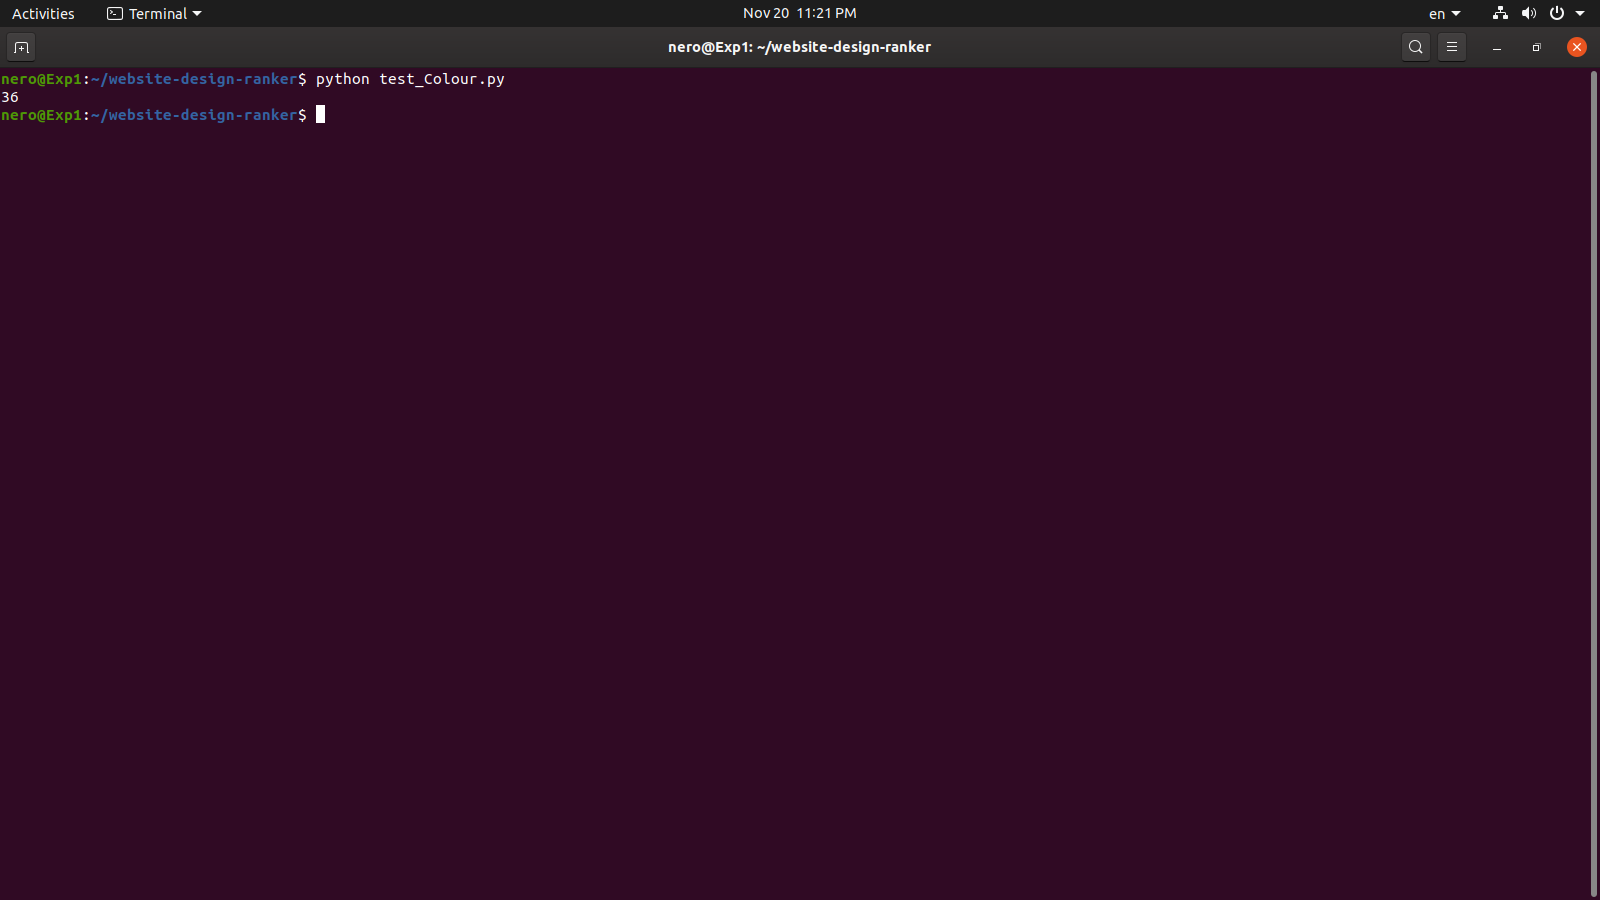
\includegraphics[scale=.3]{colourtest.png}
\end{figure}
\end{frame}
\begin{frame}
\frametitle{Data Flow Diagram}
\begin{flushleft}
	\centerline{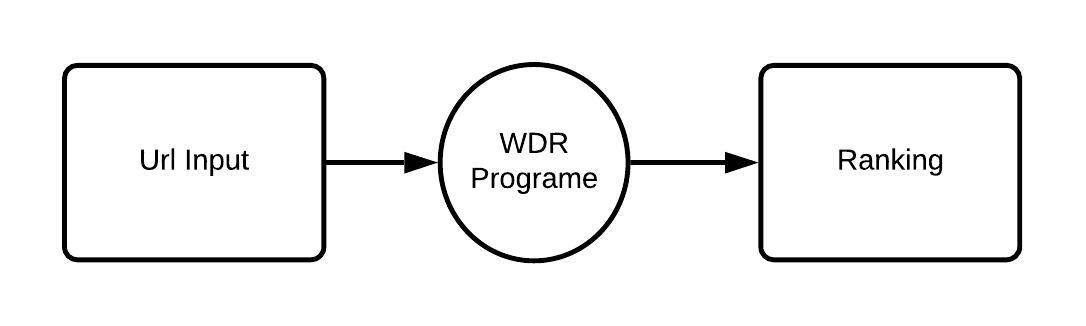
\includegraphics[scale=1.2]{image/level_0_dfd.jpeg}}
\end{flushleft}
\end{frame}
\subsection{Data Flow Diagram - Level 1}
\begin{frame}
\frametitle{Future Work}
	\begin{itemize}
\item The next parameter grid based ranking is to be implemented and an automatic rank updating mechanisum using computer vision.This will increase the efficiency of ranking thus it becomes more acceptable and accurate.
	\end{itemize}
\end{frame}
	\begin{frame}{Conclusion}
		\begin{itemize}
			\item Here we can see the logical differences in the approaches that our algorithm takes versus any existing methods.
			\item Our method relies on an objective and automated method that is consistent in nature as opposed to the subjective methods of the existing methods.
		\end{itemize}
	\end{frame}
	\begin{frame}
		\frametitle{\LARGE \textbf{References}}
		\begin{itemize}
			\item [1] - Google Page Layout Algorithm: Everything You Need to Know 
			"https://www.searchenginejournal.com/google-algorithm-history/page-layout/close"
			\item [Fig:1] - https://cdn.searchenginejournal.com/wp-content/uploads/2017/10/google-algorithm-above-the-fold-380x238.png
		
		\end{itemize}
	\end{frame}
\end{document}
